\documentclass[journal,article,submit,moreauthors,algorithms]{Definitions/mdpi} 		
\usepackage{palatino}
\usepackage{graphicx}
\usepackage[english]{babel}
%\usetikzlibrary{plotmarks}
%\pgfplotsset{compat=1.16}
\usepackage{algorithm}
\usepackage{algpseudocode}
\usepackage{subcaption}
\usepackage{tikz}
\setlength{\textfloatsep}{0pt}

\firstpage{1} 
\makeatletter 
\setcounter{page}{\@firstpage} 
\makeatother
\pubvolume{1}
\issuenum{1}
\articlenumber{0}
\pubyear{2023}
\copyrightyear{2023}
%\externaleditor{Academic Editor: Firstname Lastname}
\datereceived{ } 
\daterevised{ } % Comment out if no revised date
\dateaccepted{ } 
\datepublished{ } 
%\datecorrected{} % For corrected papers: "Corrected: XXX" date in the original paper.
%\dateretracted{} % For corrected papers: "Retracted: XXX" date in the original paper.
\hreflink{https://doi.org/} % If needed use \linebreak
%\doinum{}
%\pdfoutput=1 % Uncommented for upload to arXiv.org

%=================================================================
% Add packages and commands here. The following packages are loaded in our class file: fontenc, inputenc, calc, indentfirst, fancyhdr, graphicx, epstopdf, lastpage, ifthen, float, amsmath, amssymb, lineno, setspace, enumitem, mathpazo, booktabs, titlesec, etoolbox, tabto, xcolor, colortbl, soul, multirow, microtype, tikz, totcount, changepage, attrib, upgreek, array, tabularx, pbox, ragged2e, tocloft, marginnote, marginfix, enotez, amsthm, natbib, hyperref, cleveref, scrextend, url, geometry, newfloat, caption, draftwatermark, seqsplit
% cleveref: load \crefname definitions after \begin{document}

%=================================================================
% Please use the following mathematics environments: Theorem, Lemma, Corollary, Proposition, Characterization, Property, Problem, Example, ExamplesandDefinitions, Hypothesis, Remark, Definition, Notation, Assumption
%% For proofs, please use the proof environment (the amsthm package is loaded by the MDPI class).

%=================================================================
% Full title of the paper (Capitalized)
\Title{Polynomials representation using AVL Trees}

% MDPI internal command: Title for citation in the left column
\TitleCitation{Polynomial representation using AVL Trees}

% Author Orchid ID: enter ID or remove command
\newcommand{\orcidauthorA}{0009-0002-0208-4749} % Add \orcidA{} behind the author's name
%\newcommand{\orcidauthorB}{0000-0000-0000-000X} % Add \orcidB{} behind the author's name

% Authors, for the paper (add full first names)
\Author{Spiros Maggioros $^{1,\dagger}$\orcidA{} and Nikolas Fryganiotis$^{2,\dagger}$}

%\longauthorlist{yes}

% MDPI internal command: Authors, for metadata in PDF
\AuthorNames{Spiros Maggioros and Nikolas Fryganiotis}

% MDPI internal command: Authors, for citation in the left column
\AuthorCitation{Maggioros, S.;Fryganiotis, N.}
% If this is a Chicago style journal: Lastname, Firstname, Firstname Lastname, and Firstname Lastname.

% Affiliations / Addresses (Add [1] after \address if there is only one affiliation.)
\address{%
$^{1}$ \quad Affiliation 1; spirosmag@ieee.org\\
$^{2}$ \quad Affiliation 2; nikolasfryganiotis@gmail.com}

% Current address and/or shared authorship
\firstnote{National Technical University of Athens.}
\secondnote{Current address: Athens, Greece.} 
%\secondnote{These authors contributed equally to this work.}
% The commands \thirdnote{} till \eighthnote{} are available for further notes

%\simplesumm{} % Simple summary

%\conference{} % An extended version of a conference paper

% Abstract (Do not insert blank lines, i.e. \\) 

\abstract{We present a data structure based on AVL Trees, used for polynomial representation which allows insertion and deletion to be performed in $O(logn)$ and is able to return a sorted polynomial without further computation.Experimental results showed that this structure performs better for sparse polynomials as it has a much lower space complexity than other data structures used to store polynomials.}

% Keywords
\keyword{polynomials representation; space complexity; data structures; trees; algorithms } 

\begin{document}


\section{Introduction}
Polynomials exists everywhere, from computer science, biology, cryptography, to physics and robotics.They are used in calculus and numerical analysis to approximate other complex functions.Polynomials are also useful in algebra and algebraic geometry as they are used to construct polynomial rings and algebraic varieties.

There exists many balanced trees having a worst case behavior of $O(logn)$ for operations such as Search, Insert and Delete in a tree of n nodes. AVL trees were introduced by Adel'son-Vel'skii and Landis (1962), they are a special kind of binary tree that is strongly balanced.That means that the heights of the two child subtrees of any node differ by at most one.That will ensure as that the insertion will take at most $O(logn)$ time \cite{siddharth,karlton,tsakalidis} as the tree remain balanced at every insertion or deletion.Insertions and deletions may require the
tree to be rebalanced by one or more tree rotations.Taking advantage of those properties, we can create a tree-like structure for polynomial representation, which is strongly balanced and sorted with no further operations.Polynomials can be represented in many ways, using dynamic arrays or linked lists.Every data structure has it's advantages and drawbacks, but, when it comes to sparse polynomials, experimental results showed that using AVL trees, execution time is significantly reduced.
%%%%%%%%%%%%%%%%%%%%%%%%%%%%%%%%%%%%%%%%%%
\section{Related Work}

Generally, a polynomial of n-th degree $n \geq 0$ can be represented as : \[\sum_{i=0}^{n} a_ix^i = a_0 + a_1 \cdot x + a_2\cdot x^2 + ... + a_n \cdot x^n\]
One alternative representation of that polynomial consists of ordered pairs: 
\[ [(a_0, 0), (a_1, 1), ..., (a_n, n)]\].Each $a_i$ represents the coefficient of the i-th power of x.Note that, we can have as an input a polynomial that each coefficient is $\geq$ 0, thus, $\forall i : a_i \neq 0$, or not.For every operation that we explain bellow we will have 2 polynomials :\[\sum_{i=0}^{n} a_ix^i\] and \[\sum_{j=0}^{m} b_jx^j\] The most used implementation for this type of problems, is using a dynamic array.Taking advantage of the constant time insertion we can easily and very fast create a polynomial using just one array. The problem(that we carefully explain at the main result section) is that for very sparse polynomials, the space complexity is just too big as there'll be a lot of empty nodes. Something that fixes this problem is using a linked list.The main advantage of a linked list is quick insertion and deletion.
The linked list is a linear data structure like arrays, but unlike arrays, elements are not stored in a contiguous location.Though we can insert a node in $O(1)$ time \cite{karimov}, we want our polynomial to be sorted, so that requires $O(n)$ insertion time complexity. Even if we don't want it to be sorted we must traverse, in the worst case, all the nodes because there could exist a node with the same exponent as the node we inserting. So the check will be :  if $W.exponent \in $ in a node P in the List  $\rightarrow P.coefficient = P.coefficient + W.coefficient$.Thus, using linked lists we can't take advantage of the constant insertion time complexity.Linked Lists and Dynamic Arrays have almost the same time complexity in every operation that we are implementing in this structure.Adding will cost at most $O(n \cdot m)$ time, as we have to iterate one list(the one with less nodes) and insert the nodes to the other one, making it slower than the tree's same operation, which will cost $O(n \cdot logm)$.Note that multiplication and evaluation will be faster using an AVL tree as multiplication's time complexity will be $O(n \cdot m \cdot logd)$ ,where d is the number of nodes in the new tree that we are returning, using an AVL tree and $O(n \cdot m \cdot d)$ using a linked list, where d is the size of the new list that we are returning, because of the linear insertion time complexity.One data structure that is rarely seen for polynomial representation is Hash Tables. Hash Table is a critical data structure which is used to store a large amount of data and provides fast amortized access. When two items with same hashing value exists, there is a collision \cite{liu}. There are different implementations to solve collisions and reduce the possibility of collisions, such as open addressing and close addressing. Hash Table offer us $O(1)$ insertion time complexity \cite{liu} and no extra space complexity making it the perfect candidate for that kind of structure as it solves the only problem that the linked list has, being able to search if a node with the same exponent exists in the hash table in constant time.The only disadvantage is that there's no way we can sort a Hash Table as this structure works by mapping keys to hash values and using the hash values as the indexes of the array to store the data.Note that, we can we can combine AVL Trees with Hash Tables to get surprising fast results as referenced in \cite{Maung} and explained in \cite{HashAVL}

%%%%%%%%%%%%%%%%%%%%%%%%%%%%%%%%%%%%%%%%%%
\section{Main Result}

AVL trees have the properties of Binary Search Trees, but, unlike them, they are strongly balanced \cite{tsakalidis}.
\medbreak
\begin{Theorem}
The height h of an AVL tree with n nodes satisfies the condition $log{_2}(n+1) < h \leq 1,440\cdot log_{2}(n+2) - 0,328$.
\end{Theorem}

\begin{proof}[Proof of Theorem 1]
The lower bound is easy to prove using the B-Trees theory as explained in \cite{B-Trees}.Lets assume that the Tree $T_h$ is an AVL tree of height $h$ that has the least amount of nodes $N_h$.It's obvious that the tree must have a subtree of height $h-1$ and that subtree will be the $T_{h-1}$.Note that, the tree will be balanced even if we have a subtree with height of $h-2$.So, because we want the least nodes we'll use the $T_{h-2}$.Thus, the number of nodes in $T_h$ is $N_h = N_{h-1} + N_{h-2} + 1$ where $h \geq 2$. We can clearly see the similarity of $N_h$ function with the recursive function of Fibonacci numbers.With induction, we can show that $N_h \geq F_{h+2} - 1. \forall h \geq 0$ where $F_k$ is the k-th Fibonacci number.Now, we will perform induction:\\
\textbf{Base Case}:\\
$N_0 = 1, F_2 = 1 \rightarrow N_0 \geq F_2 - 1$.\\
$N_1 = 2, F_3 = 2 \rightarrow N_1 \geq F_3 - 1$.\\
\textbf{Inductive hypothesis}:\\
lets assume that $N_h \geq F_{h+2} - 1$ for $h = 0,1,2,...,k$. Then $N_{h+1} = N_h + N_{h-1} + 1 \geq F_{h+2} - 1 + F_{h+1} - 1 + 1 \geq F_{h+3} - 1 \geq F_{(h+1) + 2} - 1$.\\
\textbf{Inductive step}:\\
We have to show that $N_h \geq F_{h+2} - 1 \forall h \geq 0$.We know that $F_n = \frac{1}{\sqrt{5}} \cdot (\phi^n - \hat{\phi}^n)$ where $\phi = \frac{1 + \sqrt{5}}{2}$ is the golden ratio explained here \cite{goldenratio} and $\hat{\phi} = \frac{1 - \sqrt{5}}{2} \approx -0,618$ so $|\frac{\hat{\phi}^n}{\sqrt{5}} < 1|$.Eventually, $N_h \geq F_{h+2} - 1 \implies N_h \geq \frac{\phi^{h+2}}{\sqrt{5}} - 2 \implies \sqrt{5}\cdot (N_h + 2) \geq \phi^{h+2} \implies log_{\phi}(\sqrt{5} \cdot (N_h + 2)) \geq h + 2 \implies h \leq log_{\phi}(N_h + 2) + log_{\phi}(\sqrt{5} - 2) \implies h \lesssim 1,440 \cdot log_2(N_h + 2) - 0.328$.Thus, we showed that the height of a balanced AVL Tree with n nodes is $\theta(logn)$.
\end{proof}

The insertion of a value in an AVL tree is a procedure that consists of 2 parts. First and foremost, the value is being inserted in the tree using the BST insertion process. After the value’s inserted, it’s necessary to check if the tree is balanced or not. A tree is balanced if and only if $ |h_L- h_R| \leq 1 $ for every non empty AVL Tree $ T = \{r, T_L, T_R \} $  where $h_L$ is the height of the left subtree and $h_R$ is the height of the right subtree.Obviously, every perfectly balanced Binary search tree is an AVL tree \cite{preiss}.If the tree is not balanced after the insertion, we have to use the necessary rotation to make it balanced. Both single and double rotations take $O(1)$ time \cite{preiss}.


\begin{algorithm}[H]
    \caption{Calculate the Balance of a Tree} \label{get_balance}
    \begin{algorithmic}
    \Procedure{get\_balance()}{}   
    \State return height(root.left) - height(root.right) 
    \EndProcedure
\end{algorithmic}

\end{algorithm}

\begin{figure}[H]
\centering
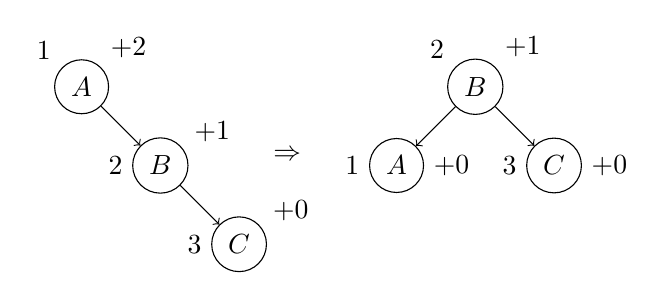
\begin{tikzpicture}[->, auto]
        \tikzstyle{vertex} = [circle,draw=black]
        \node[vertex, label = {140: $1$} , label = {45: $+2$} ] (1) at (0,0) {$A$};   
        \node[vertex, label = {180: $2$} , label = {30: $+1$}] (2) at (1, -1) {$B$};
        \node[label={above:$\Rightarrow$},rotate=45] at (3,-1.15) {};
        \node[vertex, label = {180: $3$}, label = {30: $+0$}] (3) at (2,-2) {$C$};
        \node[vertex, label = {140: $2$} , label = {45: $+1$} ] (4) at (5,0) {$B$};   
        \node[vertex, label = {180: $1$} , label = {0: $+0$}] (5) at (4, -1) {$A$};
        \node[vertex, label = {180: $3$}, label = {0: $+0$}] (6) at (6,-1) {$C$};
        \path   
                (1) edge (2)
                (2) edge (3)
                (4) edge (5)
                (4) edge (6);
\end{tikzpicture}
\label{fig:1}
\caption{Right-Right Rotation \cite{siddharth}. Let's assume the balance factor of a node $P$ is 2. This case is illustrated in the right column of the tree with coefficient $A$. We then look at the right sub-tree with root $N$. If the sub-tree is not leaning to the left(has a balance factor of 1, or after deletion, balance factor of 0) we can rotate the whole tree to the left to get a balanced tree. This is labeled as the Right-Right case. If the sub-tree does lean to the left (have a balance factor of -1) we can rotate the sub-tree to the right to end up in the Right-Right case.\\}
\end{figure}

\begin{algorithm}[H]
    \caption{Left Rotation on the Tree} \label{left_rotate}
    \begin{algorithmic}
    \Procedure{left\_rotate}{root}    
    \State t $\gets$ root.right
    \State u $\gets$ t.left
    \State t.left $\gets$ root
    \State root.right $\gets$ u
    \State return t
    \EndProcedure
\end{algorithmic}

\end{algorithm}

\begin{figure}[H]
\centering
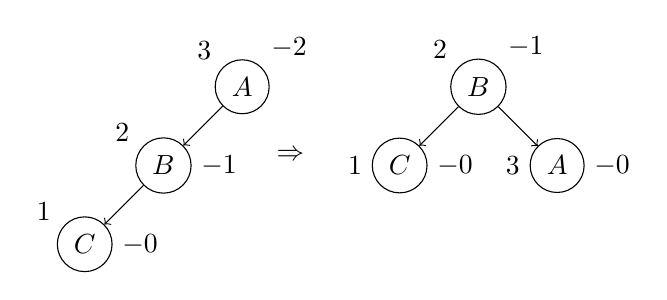
\begin{tikzpicture}[->, auto]
        \tikzstyle{vertex} = [circle,draw=black]
        \node[vertex, label = {140: $3$} , label = {45: $-2$} ] (1) at (2,0) {$A$};   
        \node[vertex, label = {150: $2$} , label = {0: $-1$}] (2) at (1, -1) {$B$};
        \node[label={above:$\Rightarrow$},rotate=45] at (3,-1.15) {};
        \node[vertex, label = {150: $1$}, label = {0: $-0$}] (3) at (0,-2) {$C$};
        
        \node[vertex, label = {140: $2$} , label = {45: $-1$} ] (4) at (5,0) {$B$};   
        \node[vertex, label = {180: $1$} , label = {0: $-0$}] (5) at (4, -1) {$C$};
        \node[vertex, label = {180: $3$}, label = {0: $-0$}] (6) at (6,-1) {$A$};
        \path   
                (1) edge (2)
                (2) edge (3)
                (4) edge (5)
                (4) edge (6);
\end{tikzpicture}
\label{fig:2}
\caption{Left-Left Rotation \cite{siddharth}. Let's assume the balance factor of a node $P$ is -2. This case is illustrated in the left column of the tree with coefficient $A$. We then look at the left sub-tree with root $N$. If the sub-tree is not leaning to the right(has a balance factor of -1, or after deletion, balance factor of 0) we can rotate the whole tree to the right to get a balanced tree. This is labeled as the Left-Left case.If the sub-tree does lean to the right(have a balance factor of 1) we can rotate the sub-tree to the left to end up in the Left-Left case.\\}
\end{figure}


\begin{algorithm}[H]
    \caption{Right Rotation on the Tree} \label{right_rotate}
    \begin{algorithmic}
    \Procedure{right\_rotate}{root}    
    \State t $\gets$ root.left
    \State u $\gets$ t.right
    \State t.right $\gets$ root
    \State root.left $\gets$ u
    \State return t
    \EndProcedure
\end{algorithmic}

\end{algorithm}


In an AVL tree, each node contains information about the value, 2 pointers to the right and left and the height of the node in the tree\cite{FPO}(also see appendix B).In our case, we just have an extra variable to store our polynomial. We insert each node based on its exponent , all exponents that are included in the left subtree $T_L$ are smaller than the exponent of r and all exponents that are included in the right subtree $T_R$ are greater than the exponent of r. More specifically, $ \forall k \in T_L \rightarrow k.exponent < r.exponent $ and  $\forall k \in T_R \rightarrow k.exponent > r.exponent$. If we insert an already existed exponent, then we just add the 2 coefficients and keep the same exponent, let’s say W is the node that we want to add, if $W.exponent \in $ in a node P in the tree  $\rightarrow P.coefficient = P.coefficient + W.coefficient. $
\medbreak
In summary, the whole insertion process takes $O(logn)$ time and the tree stays balanced. This is a huge advantage in favor of the AVL Tree because it can be iterated faster and we can have the polynomial sorted by exponent without further actions(See appendix A). That’s something that we don’t have in linked lists and while he have this property in Binary Search Trees, we lose the logarithmic time complexity of the insertion process if our polynomial is ordered \cite{BST analysis}.
\begin{Theorem}
the worst case for BST search is $O(n)$.
\end{Theorem}

%% Example of a proof:
\begin{proof}[Proof of Theorem 2]
Lets suppose our BST consists of only values in increasing order, for example, lets say we have the set $S \rightarrow {0,1,2,...,n}$.After the insertions, the tree will be transformed into a Linked List, thus, the searching time complexity will go up to $O(n)$. However, if a BST is height balanced the height is $O(logn)$.
\end{proof}


\begin{algorithm}[H]
    \caption{Insert a Node} \label{insert_node}
    \begin{algorithmic}
    \Procedure{insert\_node}{root, coefficient, exponent}
    \State n $\gets$ node(coefficient, exponent)
    \If {root == NULL}
        \State return n
    \EndIf
    \If {exponent $<$ root.expon}
        \State root.left = insert(root.left, coefficient, exponent)
    \ElsIf {exponent $>$ root.expon}
        \State root.right = insert(root.right, coefficient, exponent)
    \Else 
        \State root.coeff $\gets$ root.coeff + a
        \State return root
    \EndIf
    \State w $\gets$ get\_balance(root)
    \If {w $>$ 1}
        \If {get\_balance(root.left) $<$ 0}
            \State root.left $\gets$ left\_rotate(root.left)
         \EndIf
         \State return right\_rotate(root)
    \ElsIf {w $<$ -1}
        \If {get\_balance(root.right) $>$ 0}
            \State root.right $\gets$ right\_rotate(root.right)
         \EndIf
         \State return left\_rotate(root)
    \EndIf
    \State return root
    \EndProcedure
\end{algorithmic}

\end{algorithm}
\medbreak
Using this structure, adding 2 polynomials will take up to $O(n\cdot \log m)$ time as we can consider that to make this operation \[\sum_{i=0}^{n} a_ix^i + \sum_{j = 0}^{m} b_jx^j\] we have to iterate through the one tree(better to iterate through the tree that have less nodes so we can take advantage of the logarithmic property) and just insert the nodes to the other one. We iterate with inorder fashion, so that will take $O(n)$ time and the insertion will take $O(\log m)$ time.
\begin{algorithm}[H]
    \caption{Add two Polynomials} \label{add}
\begin{algorithmic}
    \Procedure{add}{poly\_1, poly\_2}
    \If {poly\_1 == NULL} 
        \State return poly\_2
    \EndIf
    \If {poly\_2 == NULL} 
        \State return poly\_1
    \EndIf
    \State tmp\_poly $\gets$ poly\_1
    \For {every node n $\in$ poly\_2}
    \State tmp\_poly $\gets$ insert(root, n.coeff, n.expon)
    \EndFor
    \State return tmp\_poly
    \EndProcedure
\end{algorithmic}

\end{algorithm}
\medbreak
As for multiplying, the idea is the same, the only difference is that we are traversing both trees in inorder fashion and that will take $O(n \cdot m)$ time as we can consider that \[\sum_{i=0}^{n} a_ix^i \times \sum_{j = 0}^{m} b_jx^j = \sum_{i = 0}^{n}a_ix^i \cdot (\sum_{j = 0}^{m}b_j \cdot x_j)\]. Unfortunately, we can't have the result in one of the starting polynomials and that is why we have to create a new tree to store the result. Inserting the nodes to the new tree will take $O(\log d)$ and that is making multiplication's time complexity $O(n \cdot m \cdot logd)$ where d is the number of nodes of the new tree.
\begin{algorithm}[H]
    \caption{Multiply two Polynomials} \label{multiply}
    \begin{algorithmic}
    \Procedure{multiply}{poly\_1, poly\_2}    
    \If {poly\_1 == NULL or poly\_2 == NULL}
        \State return NULL
    \EndIf
    \State poly $\gets$ NULL
    \For {every node n $\in$ poly\_2}
        \State tmp\_poly $\gets$ NULL
        \For {every node m $\in$ poly\_1}
            \State tmp\_poly $\gets$ insert(tmp\_poly, m.coeff $\cdot$ n.coeff, m.expon + n.expon)
        \EndFor
        \State poly $\gets$ add(poly, tmp\_poly)
    \EndFor
    \State return poly
    \EndProcedure
\end{algorithmic}

\end{algorithm}

A more modern version for multiplication of polynomials is using FFT(Fast Fourier Transform).Using FFT, the multiplication time complexity comes down to $\theta(n \cdot logn)$.The downside of using FFT is that, to construct the polynomial using an array, insertion's time complexity is $O(n)$ as we have to iterate through every node to check if there exist a same exponent as the one we insert.Note that, we can't use the indexes of the array as exponents, because then, there's a probability of empty nodes between used nodes, thus, FFT will not work properly.To fix this, we have to insert the nodes like an array, making the insertion's time complexity $O(n)$, which is disappointing.
Let $p(x) = a_0 + a_1x + a_2x^2 + ... + a_{n-1}x^{n-1}$ be our polynomial.Thus, let $a = (a_0, a_1, ..., a_{n-1}) \in C^n$ the set of coefficients and $DFT_n(a) = (\hat{a_0}, \hat{a_1}, ..., \hat{a_{n-1}})$ where \[\hat{a_k} = \sum_{j=0}^{n-1}a_j \cdot e^{\frac{2ikj \cdot \pi}{n}} = \sum_{j = 1}^{n - 1}a_j \cdot (\omega_n)^{kj}\]
Thus, for our polynomial \[p(\omega_n^k) = \sum_{j=0}^{n-1} a_j(\omega_n^k)^j = \hat{a_k}\] where n = sizeof(a).
We can see that with this method, time complexity is $\theta(n^2)$.We can use FFT to reduce time complexity to $\theta(n \cdot logn)$.We can split the polynomial to two polynomials $p_1$ and $p_2$ with $\frac{n}{2}$ nodes each by taking the odd and even coefficients of $p$.\[p_1(x) = a_0 + a_2x^2 + ... + a_{n-2}x^{\frac{n}{2}-2}\] \[p_2(x) = a_1 + a_3x^3 + ... + a_{n-1}x^{\frac{n}{2} - 1}\]
Then, for every $x \in C$ we can evaluate A using the following formula \[p(x) = p_e(x^2) + xp_o(x^2)\]
So, instead of computing the polynomial for all n nodes at $\omega^0_n, \omega^1_n, ..., \omega^{n-1}_n$, we just have to evaluate $p_e$ and $p_o$ for $\frac{n}{2}$ nodes \cite{FFT Rec}.In short, we divided the problem into two sub-problems of size $\frac{n}{2}$.

\algnewcommand\algorithmicforeach{\textbf{for each}}
\algdef{S}[FOR]{ForEach}[1]{\algorithmicforeach\ #1\ \algorithmicdo}


\begin{algorithm}[H]
    \caption{Recursive FFT for polynomial multiplication} \label{inorder_traversal}
    \begin{algorithmic}
    \Procedure{FFT-Rec}{a}
    \State n = sizeof(a)
    \If {n == 1}
        \State return a
    \EndIf
    \State $a_e = (a_0 , a_2 , ... , a_{n-2})$
    \State $a_o = (a_1 , a_3 , ... , a_{n-1})$
    \State $p_e = FFT-Rec(a_e)$
    \State $p_o = FFT-Rec(a_o)$
    \State $\omega_n$ = $\exp{\frac{2 \cdot \pi i}{n}}$
    \State $\omega = 1$
    \For{$k=0$ to $\frac{n}{2} - 1$}
    \State $p_k = (p_e)_k + \omega(p_o)_k$
    \State $p_{j + \frac{n}{2}} = (p_e)_k - \omega(p_o)_k$
    \State $\omega = \omega\omega_n$
    \EndFor
    \State $p = (p_o , p_1 , ... , p_{n-1})$
    \State return p
    \EndProcedure
\end{algorithmic}

\end{algorithm}
The algorithm makes two recursive calls of size $\frac{n}{2}$ and takes $\theta(n)$ time to merge the result.Thus, from Master's Theorem $T(n) = 2T(\frac{n}{2}) + \theta(n) = \theta(n \cdot logn)$ \cite{Masters Theorem}.The above algorithm is well known as Cooley Tukey Algorithm \cite{Cooley Tukey,Cooley Tukey 2}. \[X_n = \sum_{k = 0}^{\frac{N}{2} - 1} x_{2n}e^{\frac{-i 2 \pi k n}{\frac{N}{2}}} + e^{\frac{-i 2 \pi n}{N}}\sum_{k=0}^{\frac{N}{2} - 1} X_{2n + 1} e^{\frac{-i 2 \pi k n}{\frac{N}{2}}} = E_k + e^{\frac{-i 2 \pi k}{N}} O_k\] for $k = 0,1,...,\frac{N}{2} - 1$.
The first part of the sum is the DFT of even-indexed part of $X_n$ and the second part is the DFT of odd-indexed part of $X_n$.Using the periodicity of the complex exponential we can easily compute \[X_{k + \frac{N}{2}} = E_k - e^{\frac{2 \pi i k}{N}} O_k\]
\medbreak
Evaluation's time complexity is $O(n)$ as we can simply traverse the tree in inorder fashion.Have in mind that each operation will return a tree that is strongly balanced and still have all of the Binary search tree properties.
\begin{algorithm}[H]
    \caption{Evaluate a Polynomial Value for an Input} \label{evaluate}
    \begin{algorithmic}
    \Procedure{evaluate}{poly, x, val}
        \If {root!=NULL}
            \State evaluate(poly.left, x, val)
            \State val $\gets$ val + poly.coeff $\cdot$ $x ^ \text{poly.expon}$
            \State evaluate(poly.right, x, val)
        \EndIf
    
    \EndProcedure
\end{algorithmic}

\end{algorithm}

\medbreak

\begin{table}[H] 
\caption{Time complexity of AVL, BST and Linked List for each operation.(See appendix C for linked list addition time complexity).\label{fig:3}}
\newcolumntype{C}{>{\centering\arraybackslash}X}
\begin{tabularx}{\textwidth}{CCCC}
\toprule
\textbf{Functions} & \textbf{AVL}	& \textbf{BST}	& \textbf{Linked List}\\
\midrule
Insert & $O(\log n)$ & $O(n)$ & $O(n)$ \\
Add & $O(n \cdot \log m)$ & $O(n \cdot m)$ & $O(n\cdot m)$  \\
Multiply & $O(n \cdot m \cdot \log d)$ & $O(n \cdot m \cdot d)$ & $O(n \cdot  m \cdot d)$ \\
Evaluate & $O(n)$ & $O(n)$ & $O(n)$ \\
\bottomrule
\end{tabularx}
\end{table}


%\begin{algorithm}[H]
    \caption{Create a New Node} \label{create_node}
    \begin{algorithmic}
    \Procedure{create\_node}{coefficient, exponent}
    \State n $\gets$ new node() 
    \State n.coeff $\gets$ coefficient
    \State n.exponent $\gets$ exponent
    \State n.height $\gets 0$
    \State n.right $\gets$ NULL
    \State n.left $\gets$ NULL
    \State return n
    \EndProcedure
\end{algorithmic}

\end{algorithm}

%\begin{algorithm}[H]
    \caption{Calculate the Height of a Node} \label{calculate_height}
    \begin{algorithmic}
    \Procedure{inorder}{root}
    \If {root == NULL}
    \State return $0$
     \Else 
     \State return 1 + $\max \{\text{height(root.left, height(root.right)}\}$
    \EndIf
    \EndProcedure
\end{algorithmic}

\end{algorithm}

%\begin{algorithm}[H]
    \caption{Calculate the Balance of a Tree} \label{get_balance}
    \begin{algorithmic}
    \Procedure{get\_balance()}{}   
    \State return height(root.left) - height(root.right) 
    \EndProcedure
\end{algorithmic}

\end{algorithm}

%\begin{algorithm}[H]
    \caption{Left Rotation on the Tree} \label{left_rotate}
    \begin{algorithmic}
    \Procedure{left\_rotate}{root}    
    \State t $\gets$ root.right
    \State u $\gets$ t.left
    \State t.left $\gets$ root
    \State root.right $\gets$ u
    \State return t
    \EndProcedure
\end{algorithmic}

\end{algorithm}

%\begin{algorithm}[H]
    \caption{Inorder traversal} \label{inorder_traversal}
    \begin{algorithmic}
    \Procedure{inorder}{root}
    \If {root!= NULL}
    \State inorder(root.left)
     \State inorder(root.right) 
    \EndIf
    \EndProcedure
    
\end{algorithmic}

\end{algorithm}


%\begin{algorithm}[H]
    \caption{Insert a Node} \label{insert_node}
    \begin{algorithmic}
    \Procedure{insert\_node}{root, coefficient, exponent}
    \State n $\gets$ node(coefficient, exponent)
    \If {root == NULL}
        \State return n
    \EndIf
    \If {exponent $<$ root.expon}
        \State root.left = insert(root.left, coefficient, exponent)
    \ElsIf {exponent $>$ root.expon}
        \State root.right = insert(root.right, coefficient, exponent)
    \Else 
        \State root.coeff $\gets$ root.coeff + a
        \State return root
    \EndIf
    \State w $\gets$ get\_balance(root)
    \If {w $>$ 1}
        \If {get\_balance(root.left) $<$ 0}
            \State root.left $\gets$ left\_rotate(root.left)
         \EndIf
         \State return right\_rotate(root)
    \ElsIf {w $<$ -1}
        \If {get\_balance(root.right) $>$ 0}
            \State root.right $\gets$ right\_rotate(root.right)
         \EndIf
         \State return left\_rotate(root)
    \EndIf
    \State return root
    \EndProcedure
\end{algorithmic}

\end{algorithm}

%\begin{algorithm}[H]
    \caption{Add two Polynomials} \label{add}
\begin{algorithmic}
    \Procedure{add}{poly\_1, poly\_2}
    \If {poly\_1 == NULL} 
        \State return poly\_2
    \EndIf
    \If {poly\_2 == NULL} 
        \State return poly\_1
    \EndIf
    \State tmp\_poly $\gets$ poly\_1
    \For {every node n $\in$ poly\_2}
    \State tmp\_poly $\gets$ insert(root, n.coeff, n.expon)
    \EndFor
    \State return tmp\_poly
    \EndProcedure
\end{algorithmic}

\end{algorithm}

%\begin{algorithm}[H]
    \caption{Multiply two Polynomials} \label{multiply}
    \begin{algorithmic}
    \Procedure{multiply}{poly\_1, poly\_2}    
    \If {poly\_1 == NULL or poly\_2 == NULL}
        \State return NULL
    \EndIf
    \State poly $\gets$ NULL
    \For {every node n $\in$ poly\_2}
        \State tmp\_poly $\gets$ NULL
        \For {every node m $\in$ poly\_1}
            \State tmp\_poly $\gets$ insert(tmp\_poly, m.coeff $\cdot$ n.coeff, m.expon + n.expon)
        \EndFor
        \State poly $\gets$ add(poly, tmp\_poly)
    \EndFor
    \State return poly
    \EndProcedure
\end{algorithmic}

\end{algorithm}

%\begin{algorithm}[H]
    \caption{Evaluate a Polynomial Value for an Input} \label{evaluate}
    \begin{algorithmic}
    \Procedure{evaluate}{poly, x, val}
        \If {root!=NULL}
            \State evaluate(poly.left, x, val)
            \State val $\gets$ val + poly.coeff $\cdot$ $x ^ \text{poly.expon}$
            \State evaluate(poly.right, x, val)
        \EndIf
    
    \EndProcedure
\end{algorithmic}

\end{algorithm}
\section{Numerical Evaluation}

To evaluate the operation and performance of the proposed
data structure in terms of time in ms, we define three types of polynomial. In case of a \emph{normal} polynomial the exponent changes by +1 to +50 each time. In case of a \emph{semi-sparse} polynomial by +1 to +500 and in a \emph{fully-sparse} polynomial by +1 to +1000. The following graphs depict the relationship between the size of the polynomial and the time in ms that took for each operation to end, at $x$ and $y$ axis respectively. As the exponents are completely randomly chosen, there's a very small chance that even a normal polynomial will be the same as a fully-sparse. Because of that, spikes appear in each graph. It is easy to note that in case of an array the size of the representation of a polynomial, i.e. the size of the array, is the same with the size of the polynomial. For example, for add and evaluate operations with polynomials of size $n$, the size of the corresponding arrays is $O(n)$, and for multiplying $O(n^2)$ \cite{ArraysAnalysis}. This bound may stand theoretically even in the case of AVL trees, but in practice things can go strongly better, as in a node insertion with an exponent that exceeds the previous maximum exponent at least 2, there is no need to create nodes step by step for every exponent less than the new node, but only one for the new polynomial term.\par

In Figure~\ref{fig:4} we add a fully-sparse polynomial with a normal polynomial. The dynamic array seems to be better at low sizes but as the size is increasing, the size $N$ of the array is growing at a faster rate than the nodes $n$ of the AVL tree. Remember that to store polynomials in a dynamic array, we have to construct an array with size = $\max_{exponents} f(x) + 1$. For example, if we have the polynomial 
\[
f(x) = 1 + x^{1000}
\] 
and 
\[
g(x) = x + x^{780}
\]
To store $(f+g)(x)$ we have to construct an array with 1001 slots, but to store $(f+g)(x)$ in an AVL tree we just need 4 nodes as 
\[
(f+g)(x) = 1 + x + x^{780} + x^{1000}.
\]
\begin{figure}[H]
\centering
\subfloat[Using AVL Tree]
{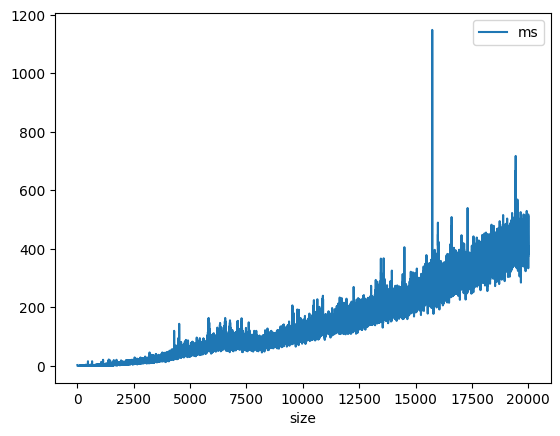
\includegraphics[width=2.3in]{pics/add_fs_normal_tree.png}
\label{fig:4a}}
\hfil
\subfloat[Using Array]{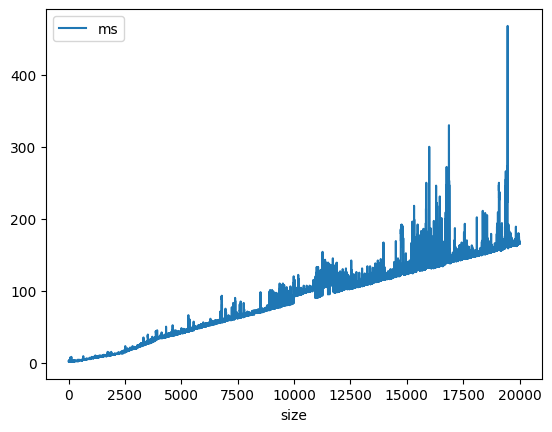
\includegraphics[width=2.3in]{pics/add_fs_normal_v}
\label{fig:4b}}
\caption{Adding a fully-sparse polynomial with a normal polynomial.}
\label{fig:4}
\end{figure} 

In Figure~\ref{fig:5} we add a semi-sparse polynomial with a normal polynomial. The results are the same as in the previous example. Contemplate that as the polynomials become less sparse, the time complexity of the tree operations become slower, as the time complexity of adding 2 polynomials is $O(n\cdot \log m)$.
\begin{figure}[H] 
\centering
\subfloat[Using AVL Tree]{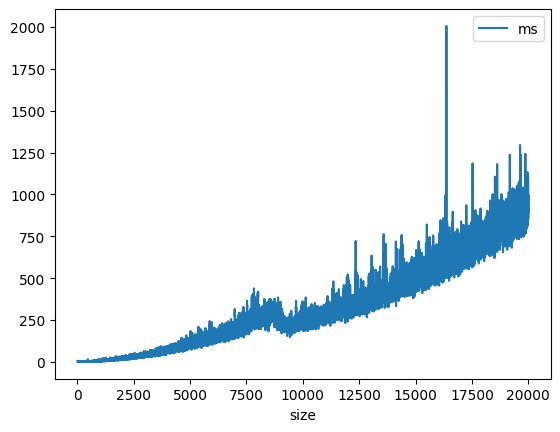
\includegraphics[width=2.3in]{pics/add_ls_normal_tree.png}
\label{fig:5a}}
\hfil
\subfloat[Using Array]{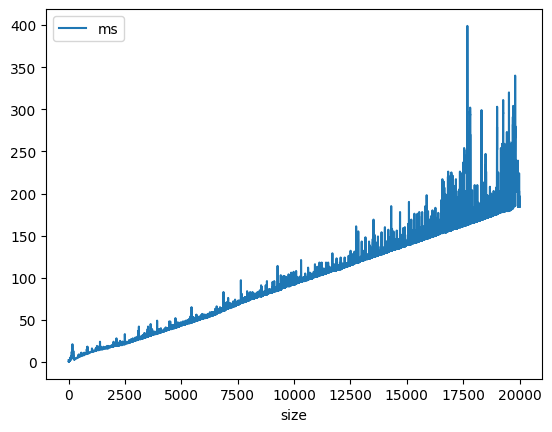
\includegraphics[width=2.3in]{pics/add_ls_normal_v.png}
\label{fig:5b}}
\caption{Adding a semi-sparse polynomial with a normal polynomial. }
\label{fig:5}
\end{figure}
In Figure~\ref{fig:6} we multiply a fully-sparse polynomial with a normal polynomial. In this case, results show that the tree is better than the dynamic array. That's because the time complexity of multiplying 2 trees is $O(n \cdot m \cdot \log d)$ where n, m is the size of the 2 trees and $d$ is the number of nodes of the new Tree that we return, the time complexity of multiplying 2 polynomials with an array is $O(n\cdot m + d)$ as we are constructing an array with size of $d = n + m - 1$ and then we iterate through the 2 arrays. Though the time complexity of the array seems better, it's not, because the product n*m of the array is growing at a faster rate than the product $n\cdot m$ of the AVL trees. Let's take the same $f$ from Figure~\ref{fig:4} and create a $g$ with 10 contiguous increasing exponents.That means that, we have to store our polynomial in an array with a size of 10 + 1001 - 1 = 1010, but, storing that in an AVL tree will just cost us 20 nodes (Figure~\ref{fig:4}).
\begin{figure}[H] 
\centering
\subfloat[Using AVL Tree]{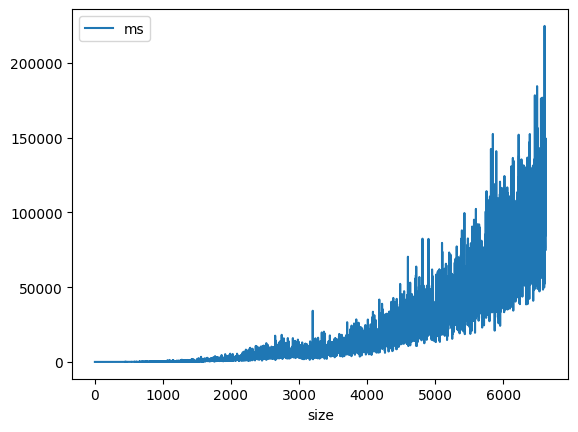
\includegraphics[width=2.3in]{pics/mult_fs_normal_tree.png}
\label{fig:6a}}
\hfil
\subfloat[Using Array]{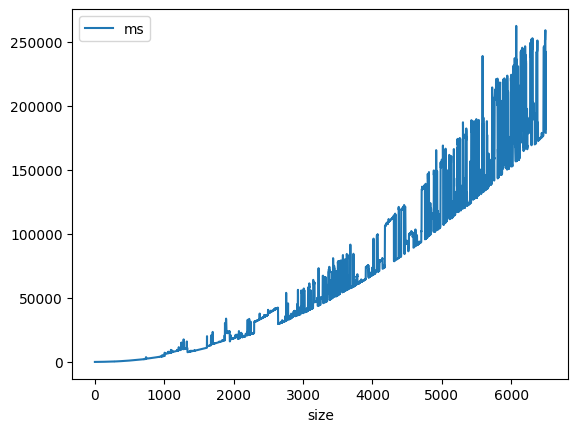
\includegraphics[width=2.3in]{pics/mult_fs_normal_v.png}
\label{fig:6b}}
\caption{Multiplying a fully-sparse polynomial with a normal polynomial.}
\label{fig:6}
\end{figure}


\begin{figure}[H] 
\centering
\subfloat[Using AVL Tree]{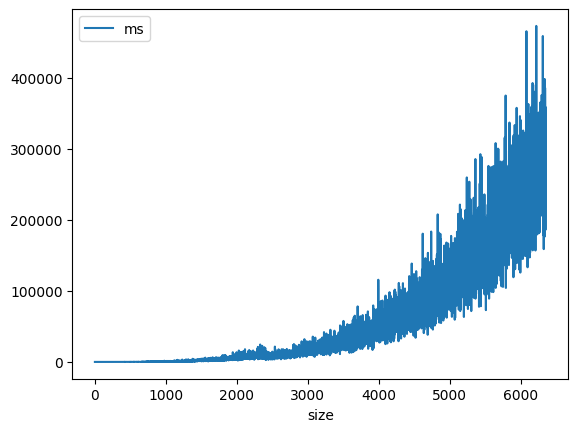
\includegraphics[width=2.3in]{pics/mult_ls_normal_tree.png}
\label{fig:7a}}
\hfil
\subfloat[Using Array]{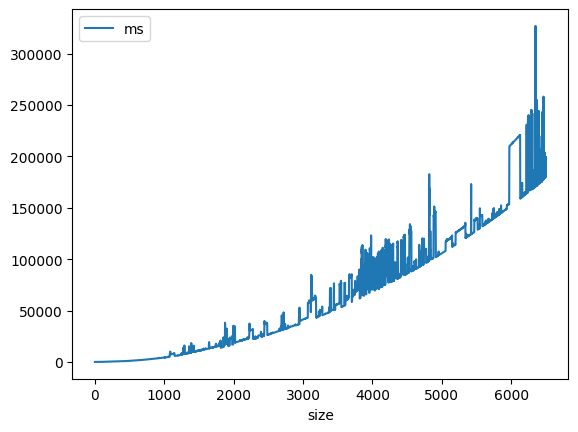
\includegraphics[width=2.3in]{pics/mult_ls_normal_v.png}
\label{fig:7b}}
\caption{Multiplying a semi-sparse polynomial with a normal polynomial. As the polynomials become less sparse, the Tree operations become slower and thus the results show that the dynamic array is better in that situation.}
\label{fig:7}
\end{figure}


\begin{figure}[H] 
\centering
\subfloat[Using AVL Tree]{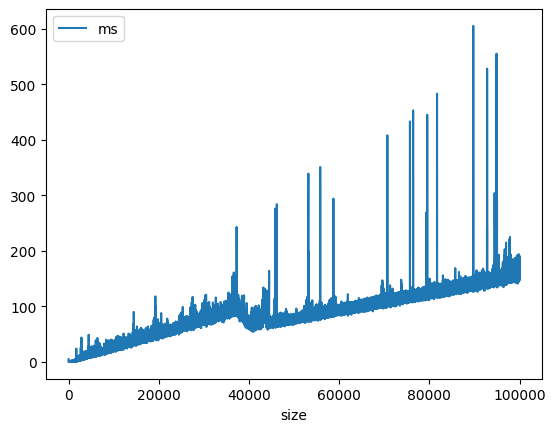
\includegraphics[width=2.3in]{pics/evaluate_ls_tree.png}
\label{fig:8a}}
\hfil
\subfloat[Using Array]{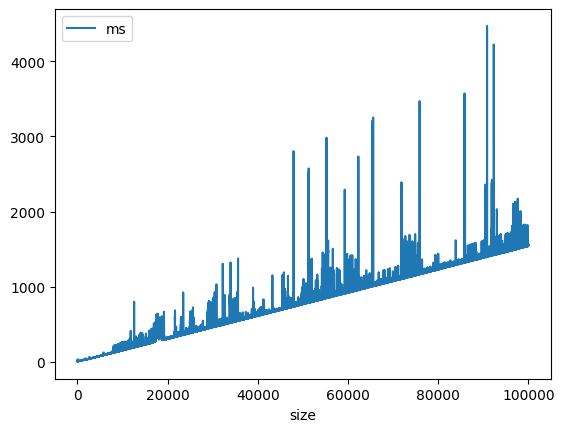
\includegraphics[width=2.3in]{pics/evaluate_ls_v.png}
\label{fig:8b}}
\caption{Evaluation of $f(x)$ for some $x \geq 10^3$ in a semi-sparse polynomial.Both operations take linear time, but, the space complexity of the AVL tree will be less than the dynamic array(Figure~\ref{fig:4}).}
\label{fig:8}
\end{figure}



\begin{figure}[H] 
\centering
\subfloat[Using AVL Tree]{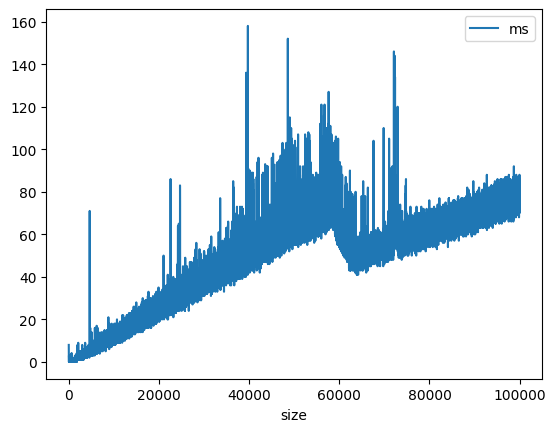
\includegraphics[width=2.3in]{pics/evaluate_fs_tree.png}
\label{fig:9a}}
\hfil
\subfloat[Using Array]{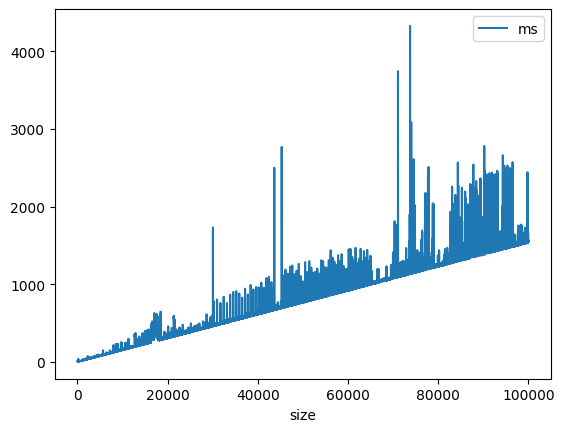
\includegraphics[width=2.3in]{pics/evaluate_fs_v.png}
\label{fig:9b}}
\caption{Evaluation of $f(x)$ for some $x \geq 10^3$ in a fully-sparse polynomial.As the polynomials become more sparse, the operations on the AVL tree become faster and on the other hand, much slower, using dynamic arrays.Have in mind that, if we have the f of Figure~\ref{fig:4}, we have to iterate 1001 slots in the array and just 2 nodes in inorder fashion for the AVL tree.}
\label{fig:9}
\end{figure}



\begin{figure}[H] 
\centering
\subfloat[Using AVL Tree]{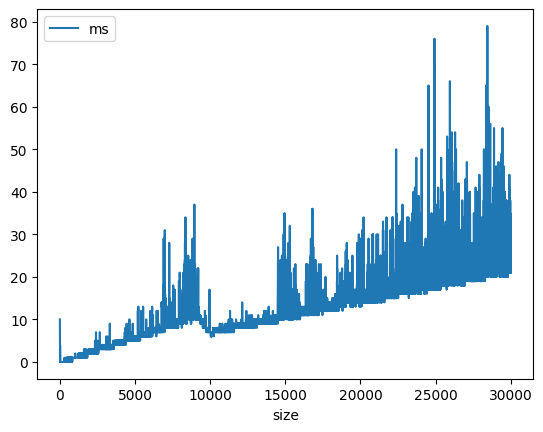
\includegraphics[width=2.3in]{pics/evaluate_normal_tre.png}
\label{fig:10a}}
\hfil
\subfloat[Using Array]{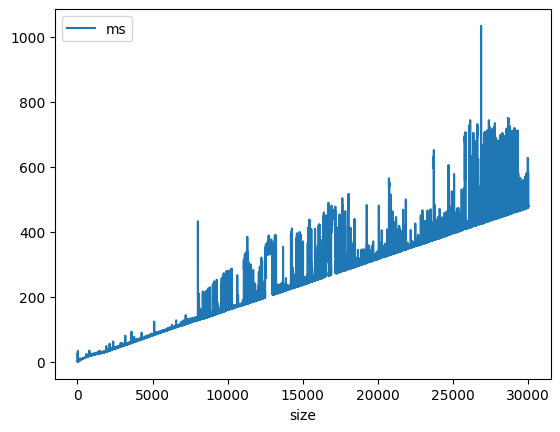
\includegraphics[width=2.3in]{pics/evaluate_normal_v.png}
\label{fig:10b}}
\caption{Evaluation of $f(x)$ for some $ x \geq 10^3$ in a normal polynomial.(Figure~\ref{fig:4})}
\label{fig:10}
\end{figure}



\begin{figure}[H] 
\centering
\subfloat[Using AVL Tree]{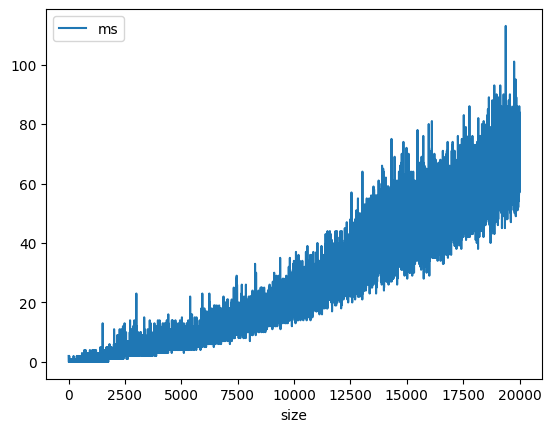
\includegraphics[width=2.3in]{pics/add_fs_ls_tree.png}
\label{fig:11a}}
\hfil
\subfloat[Using Array]{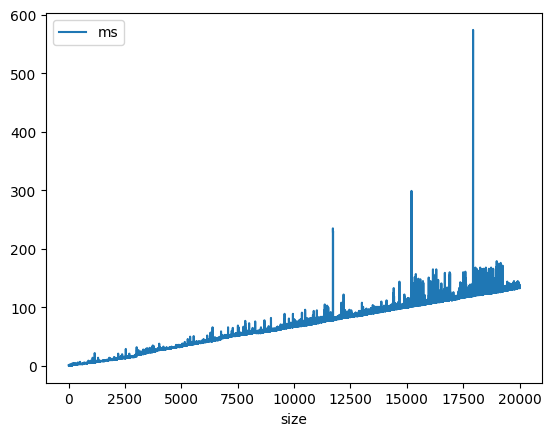
\includegraphics[width=2.3in]{pics/add_fs_ls_v.png}
\label{fig:11b}}
\caption{Adding a fully-sparse with a semi-sparse polynomial. Lets denote $n$ and $m$ the greatest exponents of each polynomial. The size of the new array has to be $\max \{n, m\}$, but, the size of the new tree will be at worst the sum of all the nodes in both trees.}
\label{fig:11}
\end{figure}



\begin{figure}[H] 
\centering
\subfloat[Using AVL Tree]{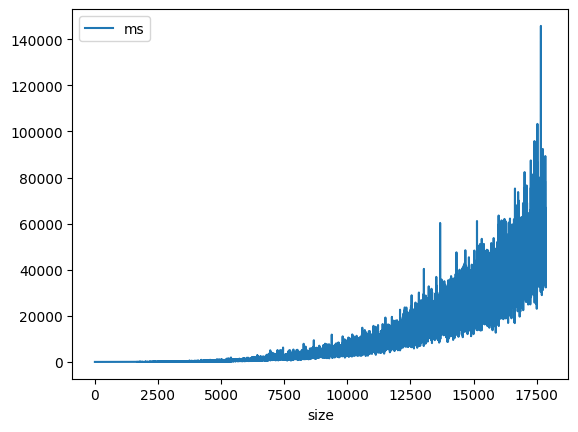
\includegraphics[width=2.3in]{pics/mult_fs_ls_tree.png}
\label{fig:12a}}
\hfil
\subfloat[Using Array]{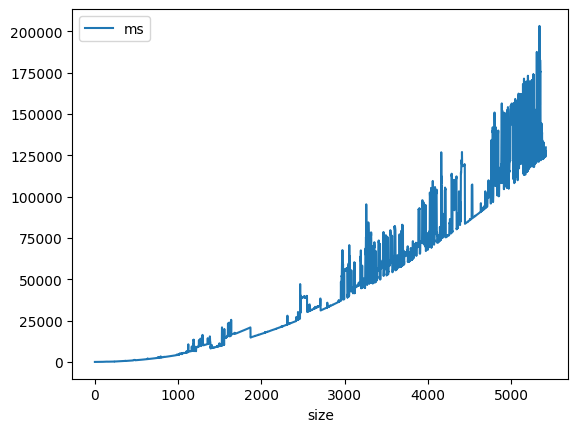
\includegraphics[width=2.3in]{pics/mult_fs_ls_v.png}
\label{fig:12b}}
\caption{Multiplying a fully-sparse polynomial with a semi-sparse polynomial.Notice that we let the multiplication run till size of almost 6000 in the array graph. The results are pretty expected as of Figure~\ref{fig:4} and Figure~\ref{fig:6}.}
\label{fig:12}
\end{figure}



\begin{figure}[H] 
\centering
\subfloat[Using AVL Tree]{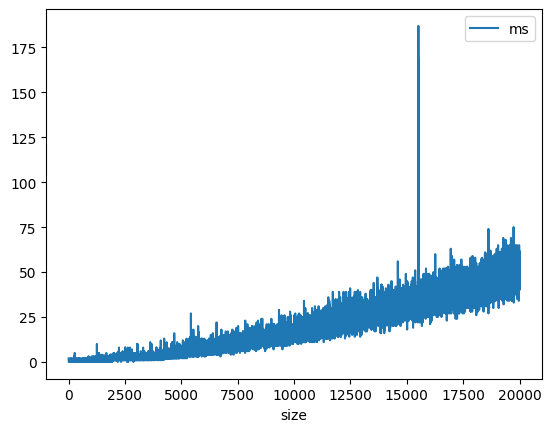
\includegraphics[width=2.3in]{pics/add_fs_fs_tree.png}
\label{fig:13a}}
\hfil
\subfloat[Using Array]{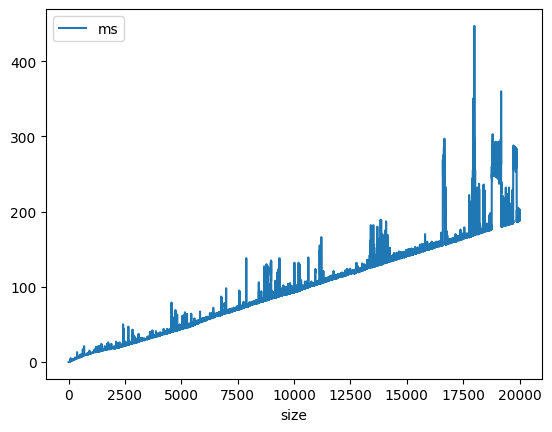
\includegraphics[width=2.3in]{pics/add_fs_fs_v.png}
\label{fig:13b}}
\caption{Adding 2 fully-sparse polynomials.(Figure~\ref{fig:4})}
\label{fig:13}
\end{figure}


\begin{figure}[H] 
\centering
\subfloat[Using AVL Tree]{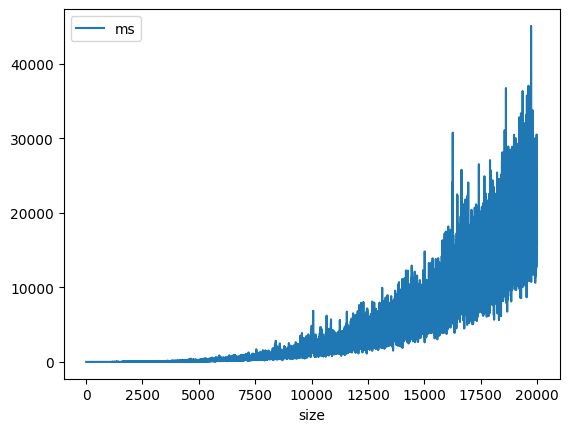
\includegraphics[width=2.3in]{pics/mult_fs_fs_tree.png}
\label{fig:14a}}
\hfil
\subfloat[Using Array]{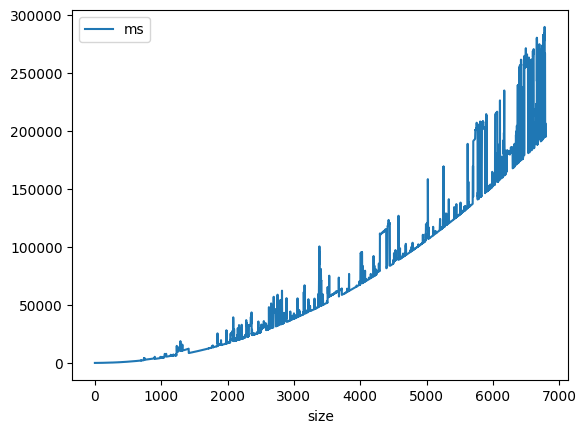
\includegraphics[width=2.3in]{pics/mult_fs_fs_v.png}
\label{fig:14b}}
\caption{Multiplying 2 fully-sparse polynomials.Notice that we let the multiplication run till size of 7000 in the array graph. Now in that case, we can clearly see the huge difference. The product $n \cdot m$ of the array is growing so much faster than the product of the number of nodes from the 2 trees. Let's take the same $f$ and $g$ from Figure~\ref{fig:4}, in order to store the multiplied polynomial in an array, we have to resize it to $d = n + m - 1$, giving us a size of 1001 + 780 - 1 = 1800.But, storing it in a tree will just cost us 4 nodes(Figure~\ref{fig:4} and Figure~\ref{fig:6})}
\label{fig:14}
\end{figure}

\vspace{6pt} 


\funding{This research received no external funding}


\informedconsent{Informed consent was obtained from all subjects involved in the study.}

\dataavailability{The data presented in this study are available on request from the corresponding author.} 

\conflictsofinterest{The authors declare no conflict of interest.} 


\appendixtitles{yes} 
\appendixstart
\appendix
\section[\appendixname~\thesection]{}
We said that, using AVL Trees we can easily represent a polynomial in it's sorted form. We used inorder traversal for every operation.
\begin{algorithm}[H]
    \caption{Inorder traversal} \label{inorder_traversal}
    \begin{algorithmic}
    \Procedure{inorder}{root}
    \If {root!= NULL}
    \State inorder(root.left)
     \State inorder(root.right) 
    \EndIf
    \EndProcedure
    
\end{algorithmic}

\end{algorithm}

As we know from Tree theory, the leftmost value is the smallest and the rightmost value is the greatest.Using recursion we can traverse the tree from left to right, getting the sorted polynomial.
\section[\appendixname~\thesection]{}
To create a node, we just created a new pointer of type "node" with the corresponding values of height, coefficient and exponent.
\begin{algorithm}[H]
    \caption{Create a New Node} \label{create_node}
    \begin{algorithmic}
    \Procedure{create\_node}{coefficient, exponent}
    \State n $\gets$ new node() 
    \State n.coeff $\gets$ coefficient
    \State n.exponent $\gets$ exponent
    \State n.height $\gets 0$
    \State n.right $\gets$ NULL
    \State n.left $\gets$ NULL
    \State return n
    \EndProcedure
\end{algorithmic}

\end{algorithm}
\section[\appendixname~\thesection]{}
We explained that Addition of 2 polynomials using a linked list is $O(n\cdot m)$.Lets assume that we have 2 polynomials, $p(x)$ and $q(x)$ that have degrees of l and m respectively.Lets also assume that the greatest exponent of $p(x)$ is smaller that the smallest exponent of $q(x)$, this means that there's no power of x common for both polynomials.We explained that in a sorted linked list insertion time complexity is $O(n)$ where n is the number of nodes in the list. Eventually, the time complexity for adding $p(x)$ and $q(x)$ will be:
\[\sum_{k=0}^{l+m-1} O(n) = O((l+m)^2)\] So, addition of polynomials using linked lists will be $O(n^2)$ for the worst case where $n = m + 1$.
%As we know from graph theory
\begin{adjustwidth}{-\extralength}{0cm}
%\printendnotes[custom] % Un-comment to print a list of endnotes

\reftitle{References}

\begin{thebibliography}{999}
% Reference 1
\bibitem[Sp.Magg(2023)]{FPO}Spiros Maggioros, Fast Polynomial Operations. Available free at: \url{http://www.github.com/spirosmaggioros/FPO}

\bibitem[AdelsonVelskii(1963)]{Velski} AdelsonVelskii, M., \& Landis, E. M. (1963). An algorithm for the organization of information. JOINT PUBLICATIONS RESEARCH SERVICE WASHINGTON DC.

\bibitem[siddharth(2014)]{siddharth}Siddharth Nair; Simran Singh Oberoi; Shubham Sharma ECE Dept, Dronacharya College of Engg AVL TREE AND ITS OPERATIONS.

\bibitem[Preiss(2016)]{preiss} Bruno R. Preiss \textit{Data Structures and Algorithms with Object-Oriented Design Patterns in C++} pp. 206-225 and pp. 361-363.

\bibitem[Wai yan Maung(2022)]{Maung}Wai yan Maung oo AVL TREE minor research.\href{https://www.academia.edu/35803329/AVL_TREE_minor_research_docx}{[CrossRef]}

\bibitem[Karimov, E.(2020)]{karimov} Karimov, E. \textit{Data Structures and Algorithms in Swift} pp. 41-54

\bibitem[Liu, D., Cui, Z., Xu, S., and Liu, H (2014)]{liu}Liu, D., Cui, Z., Xu, S., and Liu, H.An Empirical Study on the Performance of Hash Table.

\bibitem[ATHANASIOS K. TSAKALIDIS(1985)]{tsakalidis}ATHANASIOS K. TSAKALIDIS AVL-Trees for Localized Search.\href{https://www.sciencedirect.com/science/article/pii/S0019995885800346}{[CrossRef]}

\bibitem[P.L. Karlton, S.H. Fuller,R.E. Scroggs, and E.B. Kaehler (1975)]{karlton}P.L. Karlton; S.H. Fuller ; R.E. Scroggs ; E.B Kaehler Performance of Height-Balanced Trees.\href{https://www.semanticscholar.org/paper/Performance-of-height-balanced-trees-Karlton-Fuller/0c55c77491131897059f4052136b33fb3d119d63}{[CrossRef]}

\bibitem[Princeton(2021)]{BST analysis} Binary Search Trees Analysis. Princeton \href{https://algs4.cs.princeton.edu/32bst/index.php}{[CrossRef]}

\bibitem[Artur Signell, Francisco Ogando, Mats Aspnäs, Jan Westerholm (2008)]{HashAVL}Artur Signell; Francisco Ogando; Mats Aspnäs; Jan Westerholm Scalable plasma simulation with ELMFIRE using efficient data structures for process communication.\href{http://users.abo.fi/jan.westerholm/JW-46.pdf}{[CrossRef]}

\bibitem[B Lokeshwar; M Mohammed Zaid; Sk Naveen; J. Venkatesh; Lekkala Sravya(2022)]{ArraysAnalysis}B Lokeshwar; M Mohammed Zaid; Sk Naveen; J. Venkatesh; Lekkala Sravya Analysis of Time and Space Complexity of Array, Linked List and Linked Array(hybrid) in Linear Search Operation.

\bibitem[Petra Grd; Miroslav Baca (2010)]{B-Trees}Petra Grd; Miroslav Baca Analysis of B-tree data structure and its usage in computer forensics.\href{https://www.researchgate.net/publication/210381551_Analysis_of_B-tree_data_structure_and_its_usage_in_computer_forensics}{[CrossRef]}

\bibitem[ROBERT SCHNEIDER(2016)]{goldenratio} Robert Schneider Fibonacci numbers and the golden ratio \href{https://www.researchgate.net/publication/310671676_Fibonacci_numbers_and_the_golden_ratio}{[CrossRef]}

\bibitem[Uni of Toronto(2017)]{FFT Rec} Polynomial Multiplication via Fast Fourier Transforms. University of Toronto \href{http://www.cs.toronto.edu/~denisp/csc373/docs/tutorial3-adv-writeup.pdf}{[CrossRef]}

\bibitem[MIT(2021)]{Masters Theorem}Thomas H. Cormen, Charles E. Leiserson, Ronald
L. Rivest, and Clifford Stein. Introduction to Algorithms, Second Edition. MIT Press and McGraw-
Hill, 2001.

\bibitem[Stanford(1965)]{Cooley Tukey}An Algorithm for the Machine Calculation of Complex Fourier Series. Stanford \href{https://web.stanford.edu/class/cme324/classics/cooley-tukey.pdf}{[CrossRef]} 

\bibitem[Carleton(2016]{Cooley Tukey 2}Cooley Tukey FFT Algorithms. Carleton \href{http://people.scs.carleton.ca/~maheshwa/courses/5703COMP/16Fall/FFT_Report.pdf}{[CrossRef]}
\end{thebibliography}
\PublishersNote{}
\end{adjustwidth}
\end{document}